\chapter{Srovnání aplikačních rámců Angular a Vue}
Při srovnání obecných přístupů se oba rámce příliš neliší. Oba mají jako základní stavební blok komponenty a způsob použití těchto komponent je taky téměř shodný. Rámce dokáží dosáhnout podobných cílů a výsledků, ale podrobný proces, jakým dosáhnout daného cíle, se odlišuje. Velký rozdíl je také v tom, jak vývoj v aplikace v daném rámci působí.
Rámce se liší v rozdílném způsobu zpracování náhledů, Angular používá inkrementální stromovou strukturu DOM, která upravuje změněné části. Vue oproti tomu používá srovnávání virtuálních stromů DOM pro nalezení rozdílů v náhledu. Angular je více zaměřen na vývoj větších aplikací, během kterých se pracuje v týmu, protože udává jasnou strukturu. Vue je uzpůsoben tak, aby vývoj jednoduchých aplikací nebyl složitý a zároveň nabízel rozšiřitelnost pro velké aplikace s možností použít jiné nástroje.

    \section{Jazyk}
Jednou z vlastností, která ovlivňuje vývoj aplikace, je jazyk. Angular je striktně určen pro vývoj v TypeScriptu. Typescript jako takový je vhodný k objektově orientovanému programování a je lépe pochopitelný pro programátory, kteří mají zkušenost s jazyky jako je například Java, C++, PHP a další. Oproti tomu Vue umožňuje psaní kódu jak v JavaScriptu, tak v Typescriptu. Pro oba aplikační rámce existuje podrobná dokumentace, která se nachází na webových stránkách každého rámce. Typescript a Angular jako takový vyžadují v úvodu hodně nastavování, což komplikuje vývoj jednoduchých aplikací s menším množstvím funkcí. Pro vývoj takových aplikací je tak vhodnější využít spíše Vue, u něhož je základní nastavení minimální.
V demonstrační aplikaci byl v části aplikace vytvořené pomocí Vue použit jazyk JavaScript, protože její interní logika nebyla tak náročná. To se projevuje i v přehlednosti kódu v tom smyslu, že javascriptový kód je méně přehledný. Přestože bylo možné ve Vue programovat interní logiku pomocí JavaScriptu, využít JavaScript k vytvoření tak rozsáhlé interní logiky, jaká je v angularové části aplikace, by bylo velmi komplikované. Pro tyto účely tak bylo vhodnější využít Angular.

    \section{Závislosti}
Angular používá jeden velmi podstatný koncept, čímž je vkládání závislostí (Dependency Injection), které umožňuje třídám aby využívali závislosti neboli funkcionality jiné třídy. Aby Vue mohl využívat stejného konceptu, vyžaduje vložení celých komponent nebo pluginů. Toto je neefektivní, jelikož obsahují nadbytečné informace a komplikují zpracovávání kódu. 
V demonstrační aplikaci je tento koncept využit především v rámci vytvořené služby TicketService a TicketEventService, které obsahují funkce pro získávání dat z databáze. Díky tomu je možné využívat obecné části kódu a funkcí ve více komponentách současně bez nutnosti je samostatně implementovat v každé z komponent. Tento koncept je sice velmi užitečný a při studování Angularu, byl jen z komplexnějších.

    \section{Striktnost při vývoji}
To nás přivádí také k faktu, že Angular je sám o sobě robustnější, větší a má specificky definovanou strukturu. Jedná se tedy o opravdu plně vybavený aplikační rámec. Vue je spíše velmi rozsáhlá knihovna s oficiální podporou pro funkcionality potřebné pro funkční aplikační rámec. 
Vue je tedy i velmi otevřený a flexibilní, dává vývojáři možnost, aby použil vývojové postupy a technologie, které sám uzná za vhodné. Je sestaven tak, aby podporoval pouze částečné použití tohoto rámce, například pouze pro zpracování náhledu. To znamená, že je velmi dobře optimalizovaný pro tvorbu plně funkčních webových komponent. V rámci mé aplikace bylo převedení Vue části aplikace do webové komponenty velmi snadné. Nebylo k tomu potřeba žádné dodatečné nastavování a jednalo se o jednoduchý úkon.
Totéž nelze říci o rámci Angular. Angular obsahuje obrovské množství funkcí, které se díky tomu ovládají velmi podobně a celý vývoj je řízen podobnou metodologií. Pokud nebereme v potaz komplexnost Angularu, nároky na znalosti vývojáře a složité prvotní nastavování, je vývoj aplikace v Angularu velmi plynulý a přímočarý. Nevýhodou využití tohoto aplikačního rámce je ale jednoznačně to, že nedává vývojáři takovou svobodu tvořit vlastní implementace anebo vytvářet vlastní metodiku.

	\section{Souborová struktura}
Pro použití rámce Vue je potřeba pouze znalost HTML a JavaScriptu. Vue je vytvořen tak, aby byl jednoduchý na naučení i použití. Vue navíc obsahuje přehlednou a stručnou dokumentaci, která umožňuje rychlé pochopení základním principům. Vue umožňuje při tvorbě nového projektu použít grafické prostředí na spouštění sestavovacích skriptů a ukazuje přehledně parametry aplikace jako je jeho velikost a rychlost. Tyto informativní parametry dokonce rozděluje pro každou komponentu a knihovnu, díky čemuž je například snadné identifikovat kód, který aplikaci zpomaluje. 
Využití rámce Angular je v tomto ohledu oproti Vue v mnohém náročnější. Pro jeho použití je třeba ovládat HTML, TypeScript a základní mechaniku Angularu, která je komplexnější než u Vue. Angular sice nabízí pomoc při tvorbě nové aplikace pomocí jejich Angular CLI, ale oproti grafickému uživatelskému rozhraní Vue se nejedná o významné ulehčení. Pro vývoj projektu je nutné znát velké množství konceptů, kterými se Angular řídí.

    \section{Složitost učení}
Mezi drobnější rozdíly lze považovat i to, jak každý z rámců strukturuje komponenty. Angular upřednostňuje rozdělení komponent do tří souborů, a to .html šablonu obsahující náhledovou část, .ts obsahující vnitřní logiku a .css obsahující styly komponenty. Tento přístup jasně dělí komponentu na logické části. 

Vue má oproti tomu má všechny tyto části v jednom souboru s příponou .vue. Taková struktura sice šetří potřebu navigace mezi soubory s náhledem a logikou. V případě, že je komponenta rozsáhlejší, je ale dokument velmi nepřehledný a místo problému s navigací mezi soubory se objeví problém hledání místa, kde se v dokumentu nachází hledaná část aplikace. Tento přístup může být pojat jako metoda k donucení vývojáře, aby kód členil do co největšího množství komponent.

    \section{Popularita}
Popularita aplikačního rámce silně ovlivňuje vývoj aplikací. Čím je rámec populárnější, tím obsáhlejší je komunita lidí, kteří přispívají do systému vývoje knihoven a kladou otázky či nabízejí řešení týkající se práce s rámcem. Popularita také nepřímo ovlivňuje i poptávku na trhu práce. Pro srovnání popularity jsou použity statistiky ze známých a uznávaných platforem jako je Stack Overflow, npm a GitHub. V těchto grafech jsem se rozhodl zobrazit také srovnání s knihovnou React, jelikož se vedle Angularu a Vue řadí mezi nejpopulárnější javascriptové technologie a jsou vzájemně provázané.

\FloatBarrier
\begin{figure}[!htb]
\label{SOQuestions}
\centering
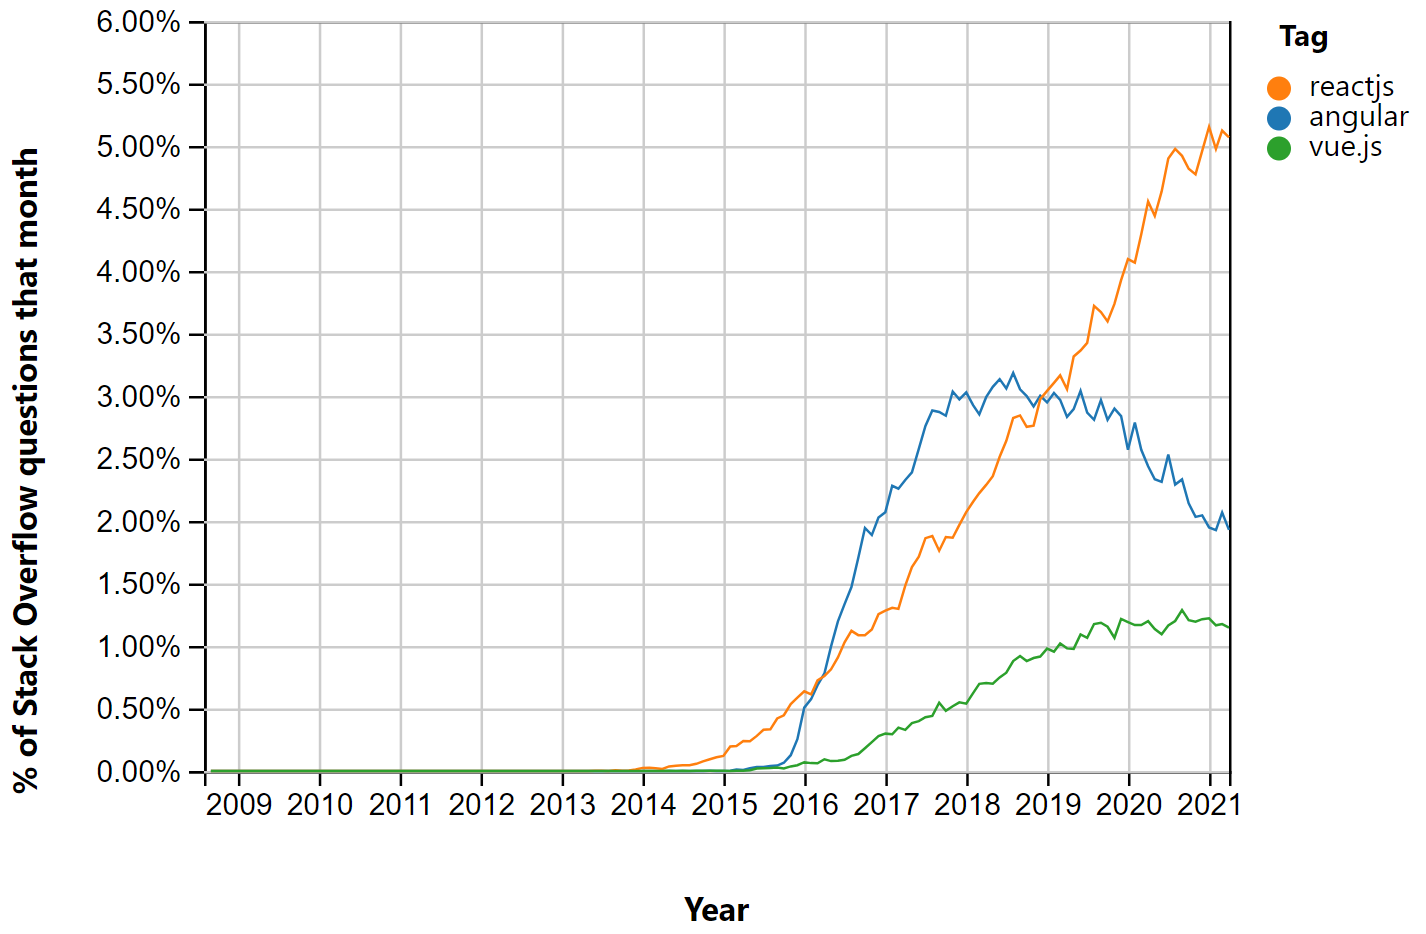
\includegraphics[width=\textwidth]{obrazky-figures/frameworkPopularityByQuestions.png}
\caption{Měsíční procentuální četnosti otázek na StackOverflow ohledně aplikačních rámců Angular, Vue, React. Převzato z \url{https://insights.stackoverflow.com/trends?tags=reactjs\%2Cvue.js\%2Cangular}}
\end{figure}
\FloatBarrier

Obrázek \ref{SOQuestions} znázorňuje měsíční procentuální četnosti otázek týkajících se daného aplikačního rámce na platformě Stack Overflow. Byla vybrána i knihovna React, protože trend úpadku Angularu nebyl tolik v prospěch Vue, jako spíše Reactu, u něhož lze pozorovat rostoucí trend.

\FloatBarrier
\begin{figure}[!htb]
\label{SOSurvey}
\centering
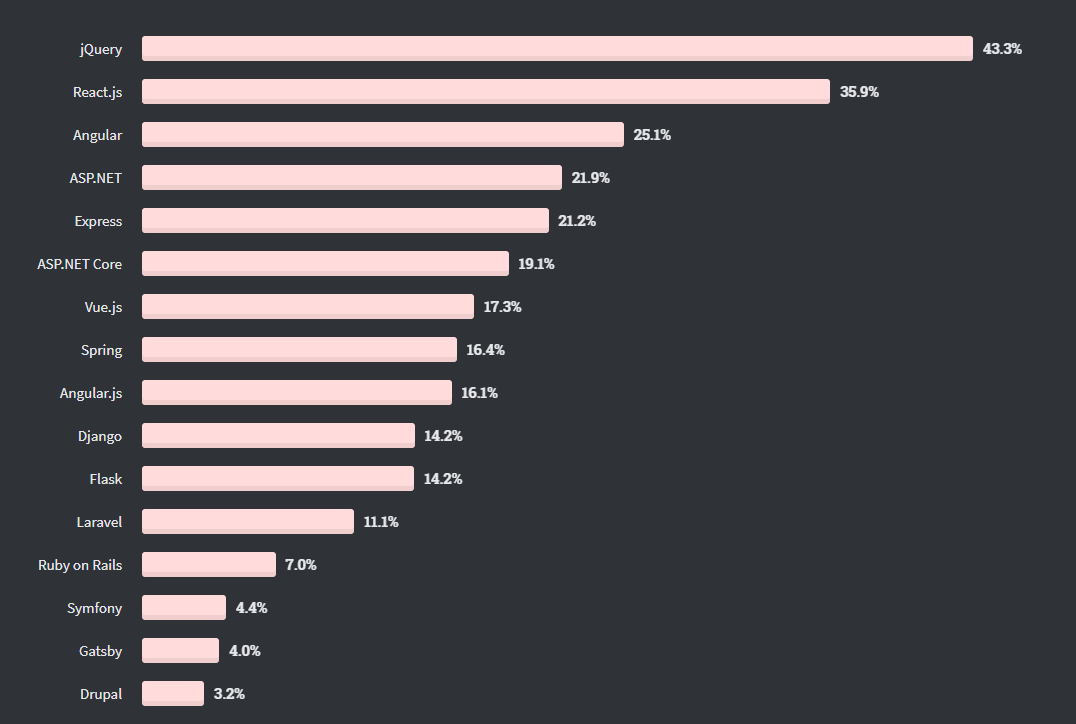
\includegraphics[width=\textwidth]{obrazky-figures/frameworkPopularityBySurvey.png}
\caption{Zastoupení využití javascriptových rámců a knihoven na základě dotazníku od společnosti StackOverflow. Převzato z \url{https://insights.stackoverflow.com/survey/2020#technology-web-frameworks}}
\end{figure}
\FloatBarrier

Stack Overflow také dělá průzkum mezi profesionálními vývojáři aplikací. Tato platforma zjišťuje, jaké technologie jsou nejvíce využívané. Na obrázku \ref{SOSurvey} je procentuální zastoupení použití daných rámců a knihoven u daných vývojářů, které vychází z dat z roku 2020. Zde Angular značně vede s 25,1 \% a Vue je na páté pozici se 17,3 \%.

\FloatBarrier
\begin{figure}[!htb]
\label{NpmDownloads}
\centering
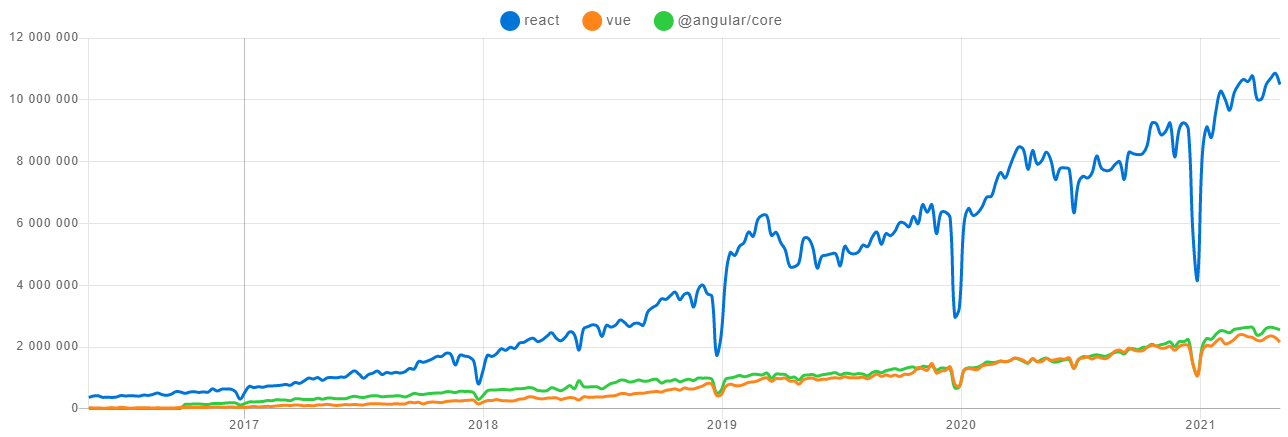
\includegraphics[width=\textwidth]{obrazky-figures/frameworkPopularityByDownloads.png}
\caption{Četnost stažení knihoven Angular, Vue a React z platformy npm. Převzato z \url{https://www.npmtrends.com/react-vs-vue-vs-@angular/core}}
\end{figure}
\FloatBarrier

V rámci platformy npm je možné sledovat počet stažení knihoven jednotlivých rámců. Kromě Angularu a Vue byl přidán také React pro lepší srovnání. Na obrázku \ref{NpmDownloads} lze pozorovat vývoj stahování těchto knihoven, přičemž je patrné, že React má nad Angularem i Vue výraznou převahu a tento trend má tendenci se časem prohlubovat. Vyšší četnost stažení knihoven Reactu může souviset s tím, že React je pouze knihovna, a tak má více použití. Angular i Vue dosahují srovnatelné četnosti stahování.

Závěrečným srovnáním je uživatelské hodnocení javascriptových aplikačních rámců na platformě GitHub. Jedná se sice pouze o subjektivní hodnocení, jež je ale přeci jen jistým ukazatelem popularity. Přední příčku zde zabírá rámec Vue, který zde obdržel více než 22 500 hvězd\cite{risingstars}. Na druhé příčce se nachází React, u kterého lze pozorovat 19 800 hvězd (tedy o 12 \% méně než Vue). Framework Angular pak zaujímá třetí pozici s 13 300 hvězdami, což je o 41 \% méně oproti Vue.


    \section{Shrnutí}
Na základě předchozího textu je patrné, že Angular je určený pro vývoj mohutnějších aplikací s komplexní vnitřní logikou. Angular svou striktností určuje chod vývoje aplikace, což podporuje týmový vývoj aplikací. Vue je oproti tomu jednoduše použitelný, lehký aplikačný rámec určený pro menší až střední projekty. Je velmi modulární a dá se dodatečně implement do jakékoliv aplikace, jak je patrné i z mnou vytvořené aplikace.